\chapter{Graphing Motion}

	\section{Introduction}
	Creating graphs of an object's motion is a useful tool for several reasons.  Graphs do all the of the following:
	\begin{itemize}
		\item Graphs allow us to visualize relationships within collected data.
		\item Graphs allow for detailed analysis, allowing us to find regression lines, slope, and area.
		\item Graphs allow for easy and intuitive extrapolation - that is, prediction of future behavior.
		\item Graphs help us to understand complex forms of motion.
		\item Graphs help us to compare different types of motion.
	\end{itemize}

In general, there are three types of graphs that physicists use routinely when studying motion of objects: \textit{Position vs Time graphs, Velocity vs Time graphs,} and \textit{Acceleration vs Time} graphs.  Using each of these types of graph, we will analyze the characteristics of different types of motion.

It may be helpful to review some math.  The formula for a line is given by:
\begin{mdframed}[backgroundcolor=orange!20!white]
\begin{equation}
	y = m x +b
\end{equation}
\end{mdframed}

where $m$ is the slope of the line and $b$ is the y-intercept.

To determine the slope of a line, use the slope formula: 
\begin{mdframed}[backgroundcolor=orange!20!white]
	\index{Slope}
	\begin{equation}
		m = \frac{rise}{run} = \frac{\Delta y} {\Delta x} = \frac{y_2-y_1}{x_2-x_1}
	\end{equation}
\end{mdframed}


\newpage
	\section{Position vs Time Graphs}
	There are some important things to know about position vs time graphs:
	\begin{enumerate}
		\item The slope of a position vs time graph is equal to the object's velocity. 
		\item Curves on a position-time graph indicate acceleration.
	\end{enumerate}
With these ideas in mind, let us examine several common types of motion.  

		\subsection{Constant Position}
		An object with a constant position will be at rest; it is not moving.  Thus, a position-time graph for a non-moving object might look something like this: 
		\begin{figure}[h]
			\centering
			\caption{Position-Time Graph for an Object at Rest}
		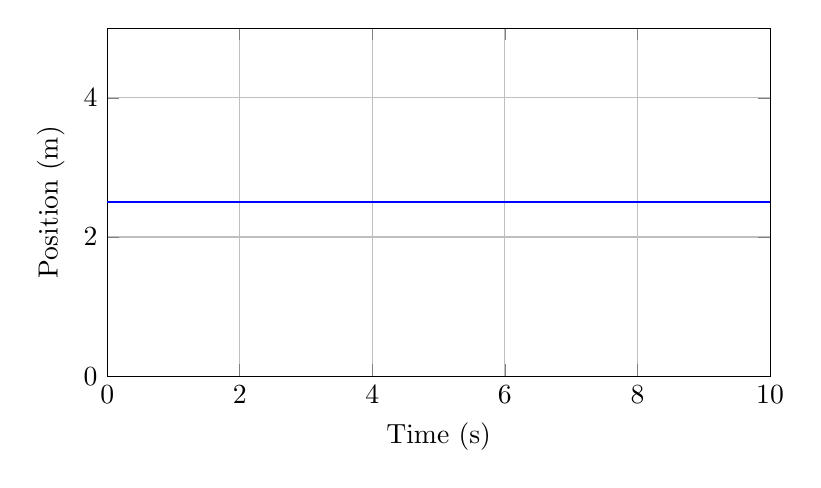
\begin{tikzpicture}
			\begin{axis}[
				xlabel={Time (s)},
				ylabel={Position (m)},
				grid=major,
				%title={Position-Time Graph for an Object at Rest},
				ymin=0, ymax=5, % Adjust the y-axis limits to show position clearly
				xmin=0, xmax=10, % Adjust the x-axis limits for the time range
				width=10cm,
				height=6cm
				]
				% Plot a horizontal line at position = 2.5 meters
				\addplot [domain=0:10, samples=100, thick, blue] {2.5};
				%\addlegendentry{$s(t) = 2.5 \text{ m}$}
			\end{axis}
		\end{tikzpicture}
		\end{figure}
	
		
		\subsection{Constant Velocity}
		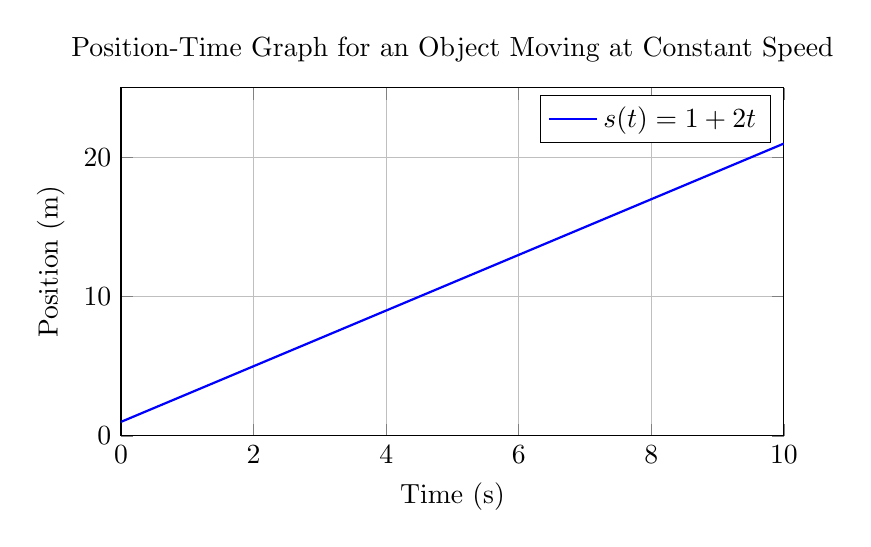
\begin{tikzpicture}
			\begin{axis}[
				xlabel={Time (s)},
				ylabel={Position (m)},
				grid=major,
				title={Position-Time Graph for an Object Moving at Constant Speed},
				ymin=0, ymax=25, % Adjust the y-axis limits to show position clearly
				xmin=0, xmax=10, % Adjust the x-axis limits for the time range
				width=10cm,
				height=6cm
				]
				% Plot the linear function for position: s(t) = 1 + 2t
				\addplot [domain=0:10, samples=100, thick, blue] {1 + 2*x};
				\addlegendentry{$s(t) = 1 + 2t$}
			\end{axis}
		\end{tikzpicture}
		
		
		
		
		
		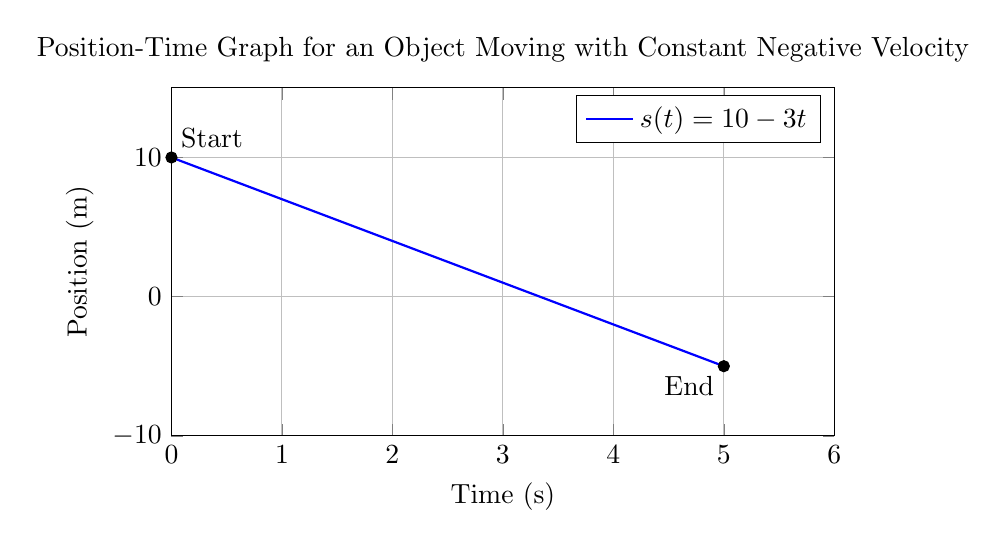
\begin{tikzpicture}
			\begin{axis}[
				xlabel={Time (s)},
				ylabel={Position (m)},
				grid=major,
				title={Position-Time Graph for an Object Moving with Constant Negative Velocity},
				ymin=-10, ymax=15, % Adjust the y-axis limits to show position clearly
				xmin=0, xmax=6, % Adjust the x-axis limits for the time range
				width=10cm,
				height=6cm
				]
				% Plot the linear function for position: s(t) = 10 - 3t
				\addplot [domain=0:5, samples=100, thick, blue] {10 - 3*x};
				\addlegendentry{$s(t) = 10 - 3t$}
				
				% Mark the starting point (0, 10)
				\addplot[mark=*] coordinates {(0, 10)};
				\node at (0, 10) [above right] {Start};
				
				% Mark the ending point (5, -5)
				\addplot[mark=*] coordinates {(5, -5)};
				\node at (5, -5) [below left] {End};
				
			\end{axis}
		\end{tikzpicture}
	
	
		
		\subsection{Constant Acceleration}
		
		
		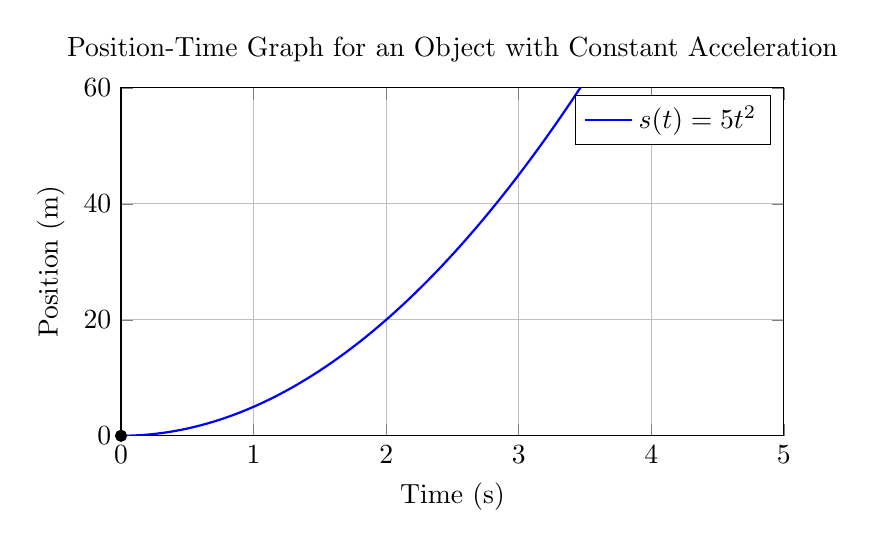
\begin{tikzpicture}
			\begin{axis}[
				xlabel={Time (s)},
				ylabel={Position (m)},
				grid=major,
				title={Position-Time Graph for an Object with Constant Acceleration},
				ymin=0, ymax=60, % Adjust the y-axis limits to show position clearly
				xmin=0, xmax=5, % Adjust the x-axis limits for the time range
				width=10cm,
				height=6cm
				]
				% Plot the quadratic function for position: s(t) = 5t^2
				\addplot [domain=0:5, samples=100, thick, blue] {5*x^2};
				\addlegendentry{$s(t) = 5t^2$}
				
				% Mark the origin point (0, 0)
				\addplot[mark=*] coordinates {(0, 0)};
				\node at (0, 0) [below right] {Start};
				
			\end{axis}
		\end{tikzpicture}
		
		
		
	\section{Velocity vs Time Graphs}
		\subsection{Constant Position}
		\subsection{Constant Velocity}
		\subsection{Constant Acceleration}
	\section{Acceleration vs Time Graphs}
		\subsection{Constant Position}
		\subsection{Constant Velocity}
		\subsection{Constant Acceleration}	
	

	


